\documentclass[a4paper,14pt]{extarticle}

% Путь до папки с общими шаблонами
\newcommand{\pathToCommonFolder}{/home/denilai/Desktop/LaTeX/Common}
% Название работы в титуле
\newcommand{\workname}{Отчет по практической работе №1}
% Название дисциплины в титуле
\newcommand{\discipline}{Теория автоматов}
% Название кафедры в титуле
\newcommand{\kafedra}{Кафедра Вычислительной техники}
% Тема работы в титуле
\newcommand{\theme}{Умножитель 4-разрядных чисел без знака}
% Должность преподавателя в титуле
\newcommand{\rang}{ассистент}
% ФИО преподавателя в титуле
\newcommand{\teacherfio}{А.~С.~Боронников}


\usepackage{tabularx}

\usepackage{booktabs}
\newcolumntype{b}{X}
\newcolumntype{s}{>{\hsize=.5\hsize}X}
\newcommand{\heading}[1]{\multicolumn{1}{c}{#1}}

% Вставка заготовки преамбулы
% Этот шаблон документа разработан в 2014 году
% Данилом Фёдоровых (danil@fedorovykh.ru) 
% для использования в курсе 
% <<Документы и презентации в \LaTeX>>, записанном НИУ ВШЭ
% для Coursera.org: http://coursera.org/course/latex .
% Исходная версия шаблона --- 
% https://www.writelatex.com/coursera/latex/5.3

% В этом документе преамбула

% Для корректного использования русских символов в формулах
% пакеты hyperref и настройки, связанные с ним, стоит загуржать
% перед загрузкой пакета mathtext



% поддержка русских букв
% кодировка шрифта
%\usepackage[T2A]{fontenc} 
\usepackage{pscyr}

% использование ненумеровонного абзаца с добавлением его в содержаниеl

\newcommand{\anonsection}[1]{\section*{#1}\addcontentsline{toc}{section}{#1}}
\newcommand{\sectionunderl}[1]{\section*{\underline{#1}}}


% настройка окружения enumerate
\usepackage{enumitem}
\setlist{noitemsep}
\setlist[enumerate]{labelsep=*, leftmargin=1.5pc}

\usepackage{hyperref}

% сначала ставить \usepackage{extsizes} % Возможность сделать 14-й шрифт
% для корректной установки полей вставлять преамбулу следует в последнюю очередь (но перед дерективой замены \rmdefault)
\usepackage[top=20mm,bottom=25mm,left=35mm,right=20mm]{geometry} % Простой способ задавать поля

\hypersetup{				% Гиперссылки
	unicode=true,           % русские буквы в раздела PDF
	pdftitle={Заголовок},   % Заголовок
	pdfauthor={Автор},      % Автор
	pdfsubject={Тема},      % Тема
	pdfcreator={Создатель}, % Создатель
	pdfproducer={Производитель}, % Производитель
	pdfkeywords={keyword1} {key2} {key3}, % Ключевые слова
	colorlinks=true,       	% false: ссылки в рамках; true: цветные ссылки
	linkcolor=red,          % внутренние ссылки
	citecolor=black,        % на библиографию
	filecolor=magenta,      % на файлы
	urlcolor=blue           % на URL
}

%%% Работа с русским языком
\usepackage{cmap}					% поиск в PDF
\usepackage{mathtext} 				% русские буквы в формулах
\usepackage[T2A]{fontenc}			% кодировка
\usepackage[utf8]{inputenc}			% кодировка исходного текста
\usepackage[english,russian]{babel}	% локализация и переносы
\usepackage{indentfirst}
\frenchspacing

%для изменения названия списка иллюстраций
\usepackage{tocloft}


\renewcommand{\epsilon}{\ensuremath{\varepsilon}}
\renewcommand{\phi}{\ensuremath{\varphi}}
\renewcommand{\kappa}{\ensuremath{\varkappa}}
\renewcommand{\le}{\ensuremath{\leqslant}}
\renewcommand{\leq}{\ensuremath{\leqslant}}
\renewcommand{\ge}{\ensuremath{\geqslant}}
\renewcommand{\geq}{\ensuremath{\geqslant}}
\renewcommand{\emptyset}{\varnothing}

% Изменения параметров списка иллюстраций
\renewcommand{\cftfigfont}{Рисунок } % добавляем везде "Рисунок" перед номером
\addto\captionsrussian{\renewcommand\listfigurename{Список иллюстративного материала}}

\newcommand{\tm}{\texttrademark\ }
\newcommand{\reg}{\textregistered\ }


%%% Дополнительная работа с математикой
\usepackage{amsmath,amsfonts,amssymb,amsthm,mathtools} % AMS
\usepackage{icomma} % "Умная" запятая: $0,2$ --- число, $0, 2$ --- перечисление

%% Номера формул
%\mathtoolsset{showonlyrefs=true} % Показывать номера только у тех формул, на которые есть \eqref{} в тексте.
%\usepackage{leqno} % Нумереация формул слева

%% Свои команды
\DeclareMathOperator{\sgn}{\mathop{sgn}}

%% Перенос знаков в формулах (по Львовскому)
\newcommand*{\hm}[1]{#1\nobreak\discretionary{}
{\hbox{$\mathsurround=0pt #1$}}{}}


% отступ для первого абзаца главы или параграфа
%\usepackage{indentfirst}

%%% Работа с картинками
\usepackage{graphicx}  % Для вставки рисунков
\graphicspath{{images/}{screnshots/}}  % папки с картинками
\DeclareGraphicsExtensions{.pdf,.png,.jpg}
\setlength\fboxsep{3pt} % Отступ рамки \fbox{} от рисунка
\setlength\fboxrule{1pt} % Толщина линий рамки \fbox{}
\usepackage{wrapfig} % Обтекание рисунков текстом

%%% Работа с таблицами
\usepackage{array,tabularx,tabulary,booktabs} % Дополнительная работа с таблицами
\usepackage{longtable}  % Длинные таблицы
\usepackage{multirow} % Слияние строк в таблице

%%% Теоремы
\theoremstyle{plain} % Это стиль по умолчанию, его можно не переопределять.
\newtheorem{theorem}{Теорема}[section]
\newtheorem{proposition}[theorem]{Утверждение}

\theoremstyle{plain} % Это стиль по умолчанию, его можно не переопределять.
\newtheorem{work}{Практическая работа}[part]


 
 
\theoremstyle{definition} % "Определение"
\newtheorem{corollary}{Следствие}[theorem]
\newtheorem{problem}{Задача}[section]
 
\theoremstyle{remark} % "Примечание"
\newtheorem*{nonum}{Решение}



%%% Программирование
\usepackage{etoolbox} % логические операторы

%%% Страница

%	\usepackage{fancyhdr} % Колонтитулы
% 	\pagestyle{fancy}
%   \renewcommand{\headrulewidth}{0pt}  % Толщина линейки, отчеркивающей верхний колонтитул
% 	\lfoot{Нижний левый}
% 	\rfoot{Нижний правый}
% 	\rhead{Верхний правый}
% 	\chead{Верхний в центре}
% 	\lhead{Верхний левый}
%	\cfoot{Нижний в центре} % По умолчанию здесь номер страницы

\usepackage{setspace} % Интерлиньяж
\onehalfspacing % Интерлиньяж 1.5
%\doublespacing % Интерлиньяж 2
%\singlespacing % Интерлиньяж 1

\usepackage{lastpage} % Узнать, сколько всего страниц в документе.

\usepackage{soul} % Модификаторы начертания


\usepackage[usenames,dvipsnames,svgnames,table,rgb]{xcolor}


\usepackage{csquotes} % Еще инструменты для ссылок

%\usepackage[style=authoryear,maxcitenames=2,backend=biber,sorting=nty]{biblatex}

\usepackage{multicol} % Несколько колонок

\usepackage{tikz} % Работа с графикой
\usepackage{pgfplots}
\usepackage{pgfplotstable}

% модуль для вставки рыбы
\usepackage{blindtext}

\usepackage{listings}
\usepackage{color}


% для поворота отдельной страницы. Использовать окружение \landscape
\usepackage{pdflscape} 
\usepackage{rotating} 


\definecolor{mygreen}{rgb}{0,0.6,0}
\definecolor{mygray}{rgb}{0.5,0.5,0.5}
\definecolor{mymauve}{rgb}{0.58,0,0.82}


% пример импорта файла
%\lstinputlisting{/home/denilai/repomy/conf/distributions}

\lstset{
	language=Python,
	basicstyle=\footnotesize,        % the size of the fonts that are used for the code
	numbers=left,                    % where to put the line-numbers; possible values are (none, left, right)
	numbersep=5pt,                   % how far the line-numbers are from the code
	numberstyle=\tiny\color{mygray}, % the style that is used for the line-numbers
	stepnumber=2,                    % the step between two line-numbers. If it's 1, each line will be numbered
	% Tab - 2 пробела
	tabsize=2,    
	% Автоматический перенос строк
	breaklines=true,
	frame=single,
	breakatwhitespace=true,
	title=\lstname 
}



% установка размера шрифта для всего документа
%\fontsize{20pt}{18pt}\selectfont
\usepackage{extsizes} % Возможность сделать 14-й шрифт

\author{Кирилл Денисов}
\title{Практическая работа №2}
\date{\today}

% установка полуторного интервала
% \usepackage{setspace}  
% \onehalfspacing

% использовать Times New Roman
\renewcommand{\rmdefault}{ftm}


\begin{document}
	\thispagestyle{empty}
	
	% Вставка первого титульного листа
	%\newcounter{withouttheme}

%\setcounter{withouttheme}{<n>} установить значение счетчика  withouttheme для определения, нужна ли тема
%    {0} - нужна
%    {1} - не нужна

%\setcounter{withoutsubmissiondate}{<n>} установить значение счетчика  withoutsubmissiondate для определения, нужна ли дата представления к защите
%     {0} - нужна
%     {1} - не нужена
\begin{center}
	\begin{figure}[h!]
		\begin{center}
		%\vspace{-10ex}
		
\includegraphics[width=0.17\linewidth]{\pathToCommonFolder/gerb}
		%\caption{}\label{pic:first}
		%	\vspace{5ex}
		\end{center}	
	\end{figure}
 	\small	МИНОБРНАУКИ РОССИИ \\
	Федеральное государственное бюджетное образовательное учреждение\\
						высшего образования\\
\normalsize					
\textbf{«МИРЭА – Российский технологический университет»\\
						РТУ МИРЭА}\\
						\noindent\rule{1\linewidth}{1pt}\\
       Институт информационных технологий\\ %\vspace{2ex}
					\kafedra\\
		\vspace{3ex}
			\large \textbf{\workname}  \\
		%\vspace{1ex}
						по дисциплине\\ «\discipline» \\
		\vspace{3ex}
		\ifnum \value{withouttheme}=0 {
			\textbf{Тема работы:}\\ <<\theme>>
		}
		\else {}
		\fi
\vspace{10ex}
\small
\begin{table}[h!]
\begin{tabular}{lp{0.6\linewidth}l}
	\textbf{Выполнил:} & студент группы ИВБО-02-19 & \\ 
	& & \studentfio \\%Д.~Н.~Федосеев\\%А.~М.~Сосунов\\%К.~Ю.~Денисов\\%И.~А.~Кремнев
	\textbf{Принял:} & \rang & \\
	& & \teacherfio \hfill\\
\end{tabular}
\end{table}
\end{center}
\ifnum \value{withoutsubmissiondate}=0 {
	\begin{flushleft}
		Работа представлена к защите <<\rule{3ex}{1pt}>>\rule{10ex}{1pt} 202\rule{1ex}{1pt} г.\hfill
	\end{flushleft}
\else {}
\fi

\normalsize
\begin{center}	
\vfill
Москва 2022
\end{center}

	
	\newpage
	\tableofcontents
	\newpage
	
\section{Общее строение автомата}
В любом устройстве обработки цифровой информации можно выделить два основных блока – операционный автомат (ОА) и управляющий автомат (УА). Операционный автомат (ОА) служит для хранения слов информации, выполнения набора микроопераций и вычисления значений логических условий, т.е. операционный автомат является структурой, организованной для выполнения действий над информацией. Микрооперации, выполняемые ОА, задаются множеством \textit{управляющих} сигналов $Y\left\{y_1,....,y_M\right\}$, с каждым из которых отождествляется определенная микрооперация.

Значения логических условий, вычисляемые в операционном автомате, отображаются множеством \textit{осведомительных} сигналов $X=\left\{x_1,...,x_L\right\}$, каждый из которых отождествляется с определенным логическим условием.

Управляющий автомат (УА) генерирует последовательность управляющих сигналов, предписанную микропрограммой и соответствующую значениям логическим условий. Управляющий автомат задает порядок выполнения действий в ОА, вытекающий из алгоритма выполнения операций. Наименование операции, которую необходимо выполнить в устройстве, определяется кодом g операции, поступающим в УА извне. 

В отличие от УА с жесткой логикой, закон функционирования которого обеспечивается определенным образом соединенными логическими элементами, в автоматах, построенных на основе ПЗУ, заданная микропрограмма реализуется в явной форме и хранится в памяти в виде последовательности управляющих слов. Управляющее слово определяет порядок работы устройства в течение одного такта и называется микрокомандой (МК). Она содержит информацию о микрооперациях, которые должны выполняться в данном такте, и (или) об адресе следующей микрокоманды.

В ходе данной практической работы был реализован автомат, выполняющий умножение 4-разрядных чисел без знака. Управляющий автомат был построен по схеме с адресным ПЗУ в последовательном варианте. Рассмотрим строение управляющего автомата. См рисунок~\ref{img:scheme}.

\begin{figure}[h!]
	\begin{center}
		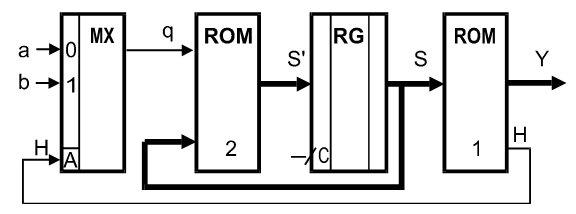
\includegraphics[width=0.8\linewidth]{line_rom}
		\caption{УА с адресным ПЗУ; последовательный вариант}
		\label{img:scheme}
	\end{center}	
\end{figure}

В конкретной реализации роль мультиплексора выполняет логический элемент ИЛИ, на входы которого подаются сигналы $CT0$~---~признак нуля в счетчике и осведомительный сигнал (признак) $H$~---~указывающий на присутствие логического ветвления в текущем месте алгоритма.
\newpage
\section{Алгоритм работы автомата}
Опишем алгоритм работы автомата с помощью блок схемы. Используем сумматор для сложения текущего значение СЧП и множимого, счетчик для подсчета обработанных разрядов и регистры для хранения и использования разрядов рассматриваемых чисел. Обозначим микрокоманды от $m_0$ до $m_4$. См. рисунок~\ref{img:algorithm}.\vspace{2ex}

\begin{figure}[h!]
	\centering
	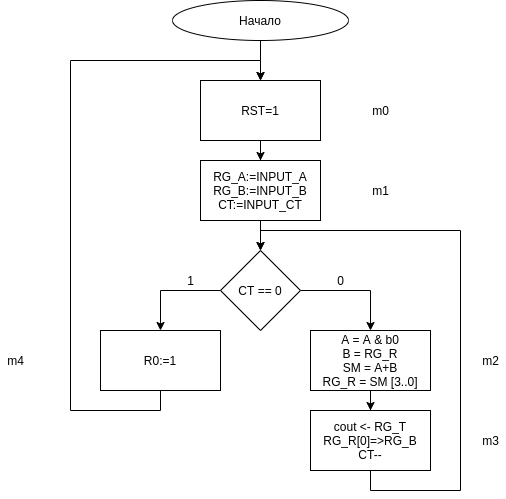
\includegraphics[width=0.8\linewidth]{algorithm}
	\caption {Алгоритм умножения двух 4-разрядных чисел}
	\label{img:algorithm}
\end{figure}

В алгоритме присутствует условие, это означает, что при реализации операционного автомата текущие значение счетчика необходимо проверять при переходе $m_0 \to m_1$ и $m_3 \to m_1$.

После построения алгоритма работы автомата следует перейти к реализации операционной части.

\section {Реализация Операционного автомата}
Построим операционный автомат, выполняющий умножение двух 4-разрядных чисел посредством использования четырех регистров, в том числе двух сдвиговых. Приведем названия и назначения каждого из регистров. См. таблицу \ref{tab:regs}.
\begin{table}[h!]
	\centering
		\begin{tabular}{|p{0.27\linewidth}|p{0.6\linewidth}|}
			\hline
			\textbf{Идентификатор} & \textbf{Назначение} \\ \hline
			$RG\_A$ & Хранит разряды множимого \\ \hline
			$RG\_B$ & Сдивговый регистр. Хранит разряды множителя \\ \hline
			$RG\_R$ & Cдвиговый регистр. Хранит разряды СЧП, служит для хранения старших разрядов результата \\ \hline
			$RG\_D$ & Сдвиговый регистр. Хранит младшие разряды результата \\ \hline
		\end{tabular}
		\caption{Регистры операционного автомата}
		\label{tab:regs}
\end{table}

Укажем необходимые признаки, которые впоследствии будут вырабатываться управляющим автоматом. См. таблицу \ref{tab:signals}.
\begin{table}[h!]
	\centering
	\begin{tabular}{|p{0.27\linewidth}|p{0.6\linewidth}|}
		\hline
		\textbf{Признак} & \textbf{Назначение} \\ \hline
		$Н$ & Указывает на условность--безусловность перехода \\ \hline
		$EMIT\_R_0$ & Сигнализирует об окончании операции умножения \\ \hline
		$LOAD\_R$ & Загрузка в регистр $RG\_R$ \\ \hline
		$RST$ & Асинхронный сброс всех элементов \\ \hline
		$COUNT\_CT$ & Загрузка счетчика. Декремент, если $DECR\_CT==1$ \\ \hline
		$DECR\_CT$ & Декремент счетчика \\ \hline
		$LOAD\_AB$ & Загрузка в регистры $RG\_A \text{ и } RG\_B$ \\ \hline
		$SHIFT\_RB$ & Сдвиг в регистрах $RG\_R \text{ и } RG\_B$ \\ \hline
	\end{tabular}
	\caption{Осведомительные сигналы (признаки)}
	\label{tab:signals}
\end{table}
Соединим все элементы в соответствии с алгоритмом задачи. См. рисунок \ref{img:oa}.

\begin{figure}[h!]
	\centering
	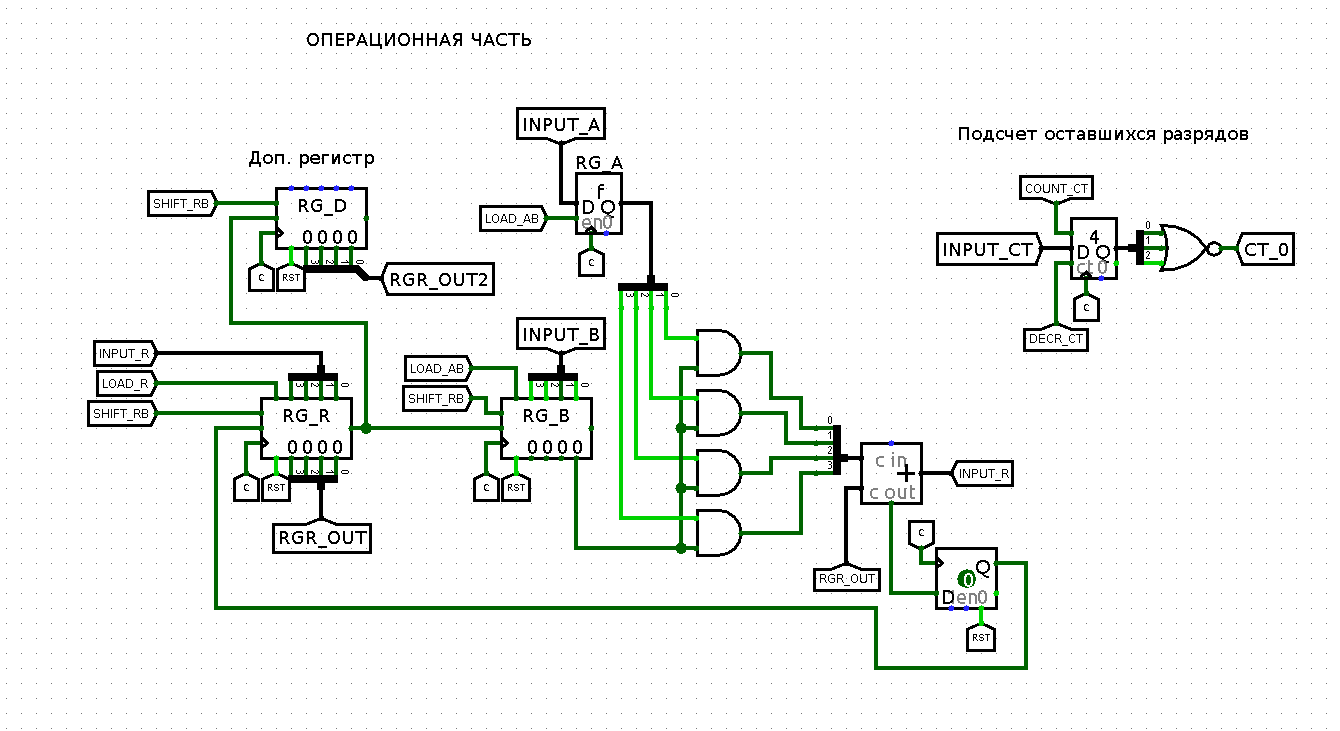
\includegraphics[width=\linewidth]{OA}
	\caption {Схема операционного автомата}
	\label{img:oa}
\end{figure}
\newpage
\section {Реализация управляющего автомата}
Приступим к построению управляющего автомата, определяющего последовательность выполнения микрокоманд для умножения двух 4-разрядных чисел. 

Определим разрядность адресного ПЗУ и ПЗУ микрокоманд. Адрес должен иметь 4 разряда, где ведущим разряд~--- текущее значение параметра \textit{CT0}. Микрокоманда представлена в виде 8 бит~--- 8 признаков, расположенных в следующем порядке: H, EMIT\_R0, LOAD\_R, RST, CONT\_CT, DECR\_CT, LOAD\_AB, SHIFT\_RB. Адрес текущей команды будет храниться в 4-разрядном регистре.


Заполним память в соответствии в алгоритмом, подключим ПЗУ и регистр последовательным способом. См рисунок \ref{img:ma}.
\begin{figure}[h!]
	\centering
	\includegraphics[width=\linewidth]{MA}
	\caption {Схема операционного автомата}
	\label{img:ma}
\end{figure}

\section{Тестирование работы автомата}
После реализации операционного и управляющего автомата следует приступить к объединению данных устройств, тестированию их совместной работы. Подключим признаки к входам соответствующих логических элементов и цифровых устройств с помощью туннелей. Добавим блок ввода исходных данных, используя контакты, блок вывода~---регистр результата и индикатор завершения операции умножения.

Проведем проверку корректности выходных результатов построенного цифрового устройства. Перемножим два наибольших 4-разрядных двоичных числа $1111_2 \ast 1111_2$ ожидая получить двоичное число $11100001_2$. Укажем входные данные, будем подавать тактовые сигналы до тех пор, пока индикатор не сообщит нам о завершении операции, сравним практические результаты с ожидаемыми. См рисунок~\ref{img:test}. Умножение выполнено корректно. Ожидаемые и полученные результаты совпадают.
\begin{figure}[h!]
	\centering
	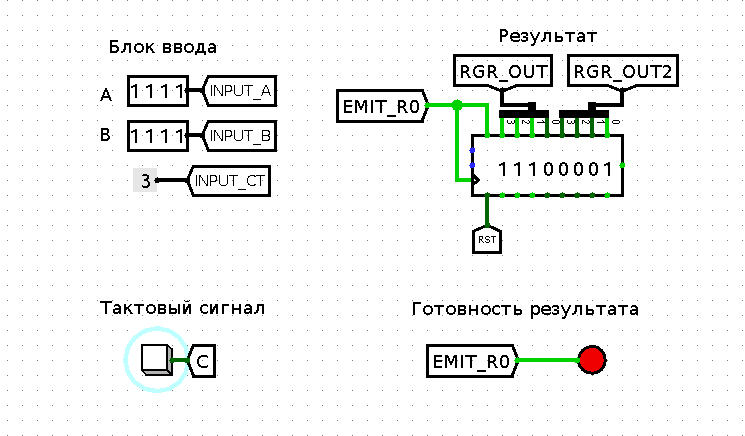
\includegraphics[width=0.7\linewidth]{test}
	\caption {Схема операционного автомата}
	\label{img:test}
\end{figure}

\newpage
\section {Вывод}
В ходе данной практической работы было рассмотрено строение и работа управляющего автомата с адресным ПЗУ. Использовав полученные знания на практике, на основе данного управляющего автомата построено вычислительное устройство (операционный и управляющий автомат), реализующее операцию умножения двух 4-разрядных чисел без знака. Работа данного устройства испытана, проверена корректность полученных результатов. 


\end{document}


